\section{How the numbers were obtained}
\label{app:method}

\subsection{Flight model and Fluent points}

The trajectory comes from the Python design tool (report~2), flown with the nose of each design. Along it,
\begin{equation}
q = \tfrac12\,\rho_\infty V^2 = \tfrac12\,\gamma\,p_\infty M^2, \qquad
T_0 = T_\infty\left(1 + \tfrac{\gamma - 1}{2}\,M^2\right).
\end{equation}
Nominal day: \SI{\val{pad-T}}{K} on the pad, propellant mass from the total impulse. Hot day:
\SI{\val{pad-Thot}}{K} on the pad and the LVO masses.

The three Fluent runs use the free stream of design~A's nominal trajectory (Table~\ref{tab:points}).
Design~B is run at the same points, so that A and B differ by shape only (B's own burnout is at
$M = \val{B-own-burnout-M}$).

\begin{table}[H]
\centering
\caption{Free stream of the Fluent runs. Reynolds number per metre: $\rho_\infty V/\mu_\infty$.}
\label{tab:points}
\small
\begin{tabular}{@{}lccc@{}}
\toprule
 & Transonic & Supersonic & Burnout\\
\midrule
Time $t$ [s] & \val{pt-M095-t} & \val{pt-M120-t} & \val{pt-M147-t}\\
Altitude $z$ [m] & \val{pt-M095-z} & \val{pt-M120-z} & \val{pt-M147-z}\\
Mach number $M$ & \val{pt-M095-M} & \val{pt-M120-M} & \val{pt-M147-M}\\
Static pressure $p_\infty$ [Pa] & \val{pt-M095-p} & \val{pt-M120-p} & \val{pt-M147-p}\\
Static temperature $T_\infty$ [K] & \val{pt-M095-T} & \val{pt-M120-T} & \val{pt-M147-T}\\
Dynamic pressure $q$ [kPa] & \val{pt-M095-q} & \val{pt-M120-q} & \val{pt-M147-q}\\
Reynolds number per metre [$10^6$/m] & \val{pt-M095-Re} & \val{pt-M120-Re} & \val{pt-M147-Re}\\
\bottomrule
\end{tabular}
\end{table}

\begin{table}[H]
\centering
\caption{Geometry of the two noses. $L$: Haack length to the sharp apex; the \SI{4.5}{mm} spherical tip
removes $\delta$, so the curved part is $x_S = L - \delta$ long.}
\label{tab:designs}
\small
\begin{tabular}{@{}lcc@{}}
\toprule
 & A (baseline) & B (backup)\\
\midrule
Profile & LV-Haack ($C = 1/3$) & Von K\'arm\'an ($C = 0$)\\
$L$ / $\delta$ [mm] & \val{A-L} / \val{A-delta} & \val{B-L} / \val{B-delta}\\
Curved part $x_S$ + coupler $c$ [mm] & \val{A-xS} + \val{A-c} & \val{B-xS} + \val{B-c}\\
Fineness $L/D$ & \val{A-fineness} & \val{B-fineness}\\
\bottomrule
\end{tabular}
\end{table}

\subsection{Drag}
\label{app:dragmethod}

The axial force is integrated over the Fluent wall faces, with $r$ the local radius:
\begin{equation}
F_p = \sum (p_w - p_\infty)\,2\pi r\,\mathrm{d}r, \qquad
F_v = \sum \tau_w\,2\pi r\,\mathrm{d}x, \qquad
C_D = \frac{F_p + F_v}{q\,A_{ref}}, \quad A_{ref} = \pi R^2 = \SI{0.025447}{m^2}.
\end{equation}
The sums reproduce Fluent's own force report to \SI{0.1}{N}. The net pressure force of the sealed nose
(Table~\ref{tab:axial}) is $\sum (p_w - p_{in})\,2\pi r\,\mathrm{d}r = F_p + (p_\infty - p_{in})\,A_{ref}$.

The flight model (report~2) adds a wave drag from Euler simulations and a flat-plate friction,
\begin{equation}
C_{D,n}(M) = C_{D,w}(M) + C_f\,\frac{S_{wet}}{A_{ref}}, \qquad
C_{D,w}(M) = C_{D,w}(1.1)\,s^2(3 - 2s), \quad s = \frac{M - M_{on}}{1 - M_{on}} \in [0, 1]
\end{equation}
below $M = 1.1$. Report~2 used $M_{on} = 0.8$, which gave 2.6 times Fluent's drag at $M = 0.95$
(\val{A-cdold-M095} against \val{A-cd-M095}). With $M_{on} = 0.94$ the model matches Fluent at all three
points:
\begin{center}\small
\begin{tabular}{@{}lccc@{}}
\toprule
Fluent / model $- 1$ & $M = 0.95$ & 1.20 & \val{pt-M147-M}\\
\midrule
A & \val{A-dcd-M095}\,\% & \val{A-dcd-M120}\,\% & \val{A-dcd-M147}\,\%\\
B & \val{B-dcd-M095}\,\% & \val{B-dcd-M120}\,\% & \val{B-dcd-M147}\,\%\\
\bottomrule
\end{tabular}
\end{center}
The change raises the apogee by \SI{7}{m} (A) and \SI{1}{m} (B). Along the flight,
$D_n(t) = q(t)\,A_{ref}\,C_{D,n}\bigl(M(t)\bigr)$, with the friction of a \SI{20}{\micro m} rough wall and
the coupler included.

\subsection{Side force}

Under a small angle of attack $\alpha$ [rad], slender-body theory gives, with $S(x) = \pi r(x)^2$ and $V_n$
the volume of the nose,
\begin{equation}
\frac{\mathrm{d}N}{\mathrm{d}x} = 2\,q\,\alpha\,\frac{\mathrm{d}S}{\mathrm{d}x}, \qquad
N = 2\,q\,A_{ref}\,\alpha, \qquad
x_{CP} = x_S - \frac{V_n}{A_{ref}}.
\end{equation}

\subsection{Heating}
\label{app:heatmethod}

From the two Fluent runs at burnout (adiabatic wall, wall at \SI{300}{K}):
\begin{equation}
h(x) = \frac{q_w(x)}{T_{aw}(x) - \SI{300}{K}}, \qquad r(x) = \frac{T_{aw}(x) - T_\infty}{T_0 - T_\infty}.
\end{equation}
The recovery factor $r$ is \val{A-recovery} (A) and \val{B-recovery} (B) on the shell.

The flight model of report~1 uses
\begin{gather}
h_s = 0.763\,\mathrm{Pr}^{-0.6}\sqrt{\rho_s\,\mu(T_0)\,\frac{\mathrm{d}u_e}{\mathrm{d}x}}\;c_p, \quad
\frac{\mathrm{d}u_e}{\mathrm{d}x} = \frac{1}{r_n}\sqrt{\frac{2(p_0 - p_\infty)}{\rho_s}}
\quad\text{(tip, Fay--Riddell)},\\
h_t = \mathrm{St}\,\rho^* V c_p, \quad \mathrm{St} = 0.0296\,\mathrm{Re}_x^{*\,-0.2}\,\mathrm{Pr}^{-2/3},
\quad T_r = T_\infty\left(1 + r\,\tfrac{\gamma - 1}{2}M^2\right),\ r = \mathrm{Pr}^{1/3}
\quad\text{(shell, Eckert)},
\end{gather}
with $\rho^*$, $\mathrm{Re}_x^*$ at Eckert's reference temperature
$T^* = T_\infty(1 + 0.032M^2 + 0.58(T_w/T_\infty - 1))$.

At burnout the model and Fluent can be compared directly (Figure~\ref{fig:hcal}). Without any correction
the model is already within \SI{6}{\percent} of Fluent at the tip and along the shell. Three small
factors bring it onto Fluent (Table~\ref{tab:calibfull}).

\begin{figure}[H]
\centering
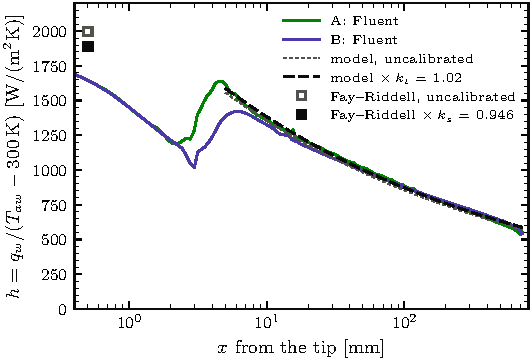
\includegraphics[width=0.75\linewidth]{fig_h_calibration}
\caption{Heat-transfer coefficient at burnout on a \SI{300}{K} wall: Fluent for A and B (smoothed between
3 and 15\,mm), the model of the shell before and after calibration (lines), and the model of the tip
before and after calibration (squares, placed at 0.5\,mm).}
\label{fig:hcal}
\end{figure}

\begin{table}[H]
\centering
\caption{Fluent against the uncalibrated model at burnout, wall at \SI{300}{K}, and the factor used in the
flight model.}
\label{tab:calibfull}
\small
\begin{tabular}{@{}lccc@{}}
\toprule
Fluent / model & A & B & Factor\\
\midrule
Heat flux at the tip & \val{A-ratio-s} & \val{B-ratio-s} & $k_s = \val{ks}$\\
$h$ along the shell, 50\,mm to shoulder (median, 10--90\,\%) & \val{A-ratio-t} (\val{A-ratio-t-lo}--\val{A-ratio-t-hi}) & \val{B-ratio-t} (\val{B-ratio-t-lo}--\val{B-ratio-t-hi}) & $k_t = \val{kt}$\\
Heat into the first \val{tip-length}\,mm (tip insert) [W] & \val{A-Qtip-fluent} / \val{A-Qtip-model} & \val{B-Qtip-fluent} / \val{B-Qtip-model} & $k_{tip} = \val{ktip}$\\
\bottomrule
\end{tabular}
\end{table}

The lumped tip insert takes its side heating at $x_{tip}/2$, which misses the high $h$ just behind the
spherical cap; with $k_s$ and $k_t$ applied it still gets 13--\SI{15}{\percent} too little heat, hence
$k_{tip}$. Fluent's recovery factor (\val{A-recovery}) is a little above the model's
$\mathrm{Pr}^{1/3} = \val{recovery-model}$, so the model's driving temperature on the shell
($T_r = \SI{\val{Tr-model}}{K}$) is 1--\SI{4}{K} below Fluent's $T_{aw}$.

With the calibrated $h$, two wall models are integrated along the trajectories:
\begin{itemize}
\item \textbf{shell}: one-dimensional conduction through the CFRP, heated outside, adiabatic inside,
\begin{equation}
\rho c\,\frac{\partial T}{\partial t} = k\,\frac{\partial^2 T}{\partial y^2}, \qquad
-k\frac{\partial T}{\partial y}\Big|_{out} = h\,(T_r - T_w), \qquad \frac{\partial T}{\partial y}\Big|_{in} = 0;
\end{equation}
run at 50\,mm for the histories of Section~\ref{sec:heating} and at 22 stations from 10\,mm to the shoulder
for the thermal profile (\file{report_720/thermal_profile.py});
\item \textbf{Al tip insert}: one temperature (aluminium conducts fast),
\begin{equation}
m\,c\,\frac{\mathrm{d}T}{\mathrm{d}t} = k_{tip}\left[0.55\,h_s A_{cap}(T_0 - T) + h_t(x_{tip}/2)\,A_{lat}(T_r - T)\right].
\end{equation}
\end{itemize}
The inside air (upper bound) is the mean inner-face temperature at 50\,mm, mid-length and shoulder, never
below the pad temperature.
